\documentclass{beamer}
\mode<presentation>
{\usetheme{Berlin}}
\usepackage[orientation=portrait,size=a0,scale=1.4]{beamerposter}

%% %%%%%%%%%%%%%%%%%%%%%%%%%%%%%%%%%%%%%%%%%%%%%%%%%%%%%%%%%%%%%%%%%%%%%%%%%%%%%
%% %%%%%%% %% %% %  %                                      %  % %% %% %%%%%%%%%%
%%%%% %% %  %                    MES COMMANDES                     %  % %% %%%%%
%%%%%%%%%% %% %% %  %                                      %  % %% %% %%%%%%% %%
%%%%%%%%%%%%%%%%%%%%%%%%%%%%%%%%%%%%%%%%%%%%%%%%%%%%%%%%%%%%%%%%%%%%%%%%%%%%% %%


\def\zzpackages{
  \usepackage[utf8]{inputenc}
  \usepackage[T1]{fontenc}
%  \usepackage[french]{babel}

  \usepackage{amsthm}
  \usepackage{amsmath}
  \usepackage{amsfonts}
  \usepackage{amssymb}

  \usepackage{xcolor}
  \usepackage{xstring}	%\ifstreqcase
}

%% %%%%%%%%%%%%%%%%%%%%%%%%%%%%%%%%%%%%%%%%%%%%%%%%%%%%%%%%%%%%%%%%%%%%%%%%%%%%%
%                              TESTS / FOR / ...                               %
%%%%%%%%%%%%%%%%%%%%%%%%%%%%%%%%%%%%%%%%%%%%%%%%%%%%%%%%%%%%%%%%%%%%%%%%%%%%% %%

% 
\def\defactive#1#2{
  \catcode`#1=13
  \begingroup
  \lcode`~=`#1
  \lowercase{\endgroup\def~}{#2}
}

\def\zifempty#1#2#3{\def\foo{#1}\ifx\foo\empty\relax#2\else#3\fi}

%% %%%%%%%%%%%%%%%%%%%%%%%%%%%%%%%%%%%%%%%%%%%%%%%%%%%%%%%%%%%%%%%%%%%%%%%%%%%%%
%                           MARGES / HYPERREF / ...                            %
%%%%%%%%%%%%%%%%%%%%%%%%%%%%%%%%%%%%%%%%%%%%%%%%%%%%%%%%%%%%%%%%%%%%%%%%%%%%% %%

\makeatletter
\gdef\@subtitle{}
\def\subtitle#1{\gdef\@subtitle{#1}}

\def\zztitre{
\begingroup\centering
{\bfseries \huge \@title}\par\vspace{.3cm}
\ifx\@subtitle\empty\else{\bfseries \Large \@subtitle}\par\vspace{.5cm}\fi
\Large \@author\par\vspace{.1cm}
\@date\zal\vspace{.3cm}\zal
\zligne\endgroup
}

\makeatother


\newcommand{\zzhyperref}{
\usepackage{hyperref}
\hypersetup{ colorlinks=true, linkcolor=blue!30!black,
citecolor=green!30!black, filecolor=magenta!30!black,
urlcolor=cyan!30!black }
}

\newcommand{\zzmarges}{
  \setlength{\textheight}{620pt}
  \addtolength{\textwidth}{2cm}
  \addtolength{\hoffset}{-1cm}
  \addtolength{\voffset}{-1cm}
  \addtolength{\marginparwidth}{0cm}
  \addtolength{\textheight}{1cm}
} 

\makeatletter
\newcommand{\zzheader}[6]{
\def\@oddhead{\vbox to 0pt{\vss\hspace{0pt} #1\hfill #2\hfill #3\kern4pt\par\kern5pt\hrule height.5pt}}
\def\@oddfoot{\vbox to 0pt{\hrule height.5pt\kern5pt\hbox to \linewidth{\kern4pt {#4}\hss {#5}\hss {#6}\kern4pt}\vss}}}
\makeatother

%%%%%%%%%%%%%%%%%%%%%%%%%%%%%%%%%%%%%%%%%%%%%%%%%%%%%%%%%%%%%%%%%%%%%%%%%%%%%%%%

\newcommand{\zligne}[1][]{
\par\zifempty{#1}%
{\hbox to \linewidth{\leaders\hrule height3pt depth-2.5pt\hfill}}%
{\hbox to \linewidth{\leaders\hrule height3pt depth-2.5pt\hfill\kern.8em #1\kern.8em\leaders\hrule height3pt depth-2.5pt\hfill}}\par
}

%%%%%%%%%%%%%%%%%%%%%%%%%%%%%%%%%%%%%%%%%%%%%%%%%%%%%%%%%%%%%%%%%%%%%%%%%%%%%%%%

\newcommand{\zal}{\par}
\newcommand{\znl}{\zal ~\zal}
\newcommand{\zguill}[2][]{«\,#2\,»}

%% %%%%%%%%%%%%%%%%%%%%%%%%%%%%%%%%%%%%%%%%%%%%%%%%%%%%%%%%%%%%%%%%%%%%%%%%%%%%%
%                             COMMANDES PRATIQUES                              %
%%%%%%%%%%%%%%%%%%%%%%%%%%%%%%%%%%%%%%%%%%%%%%%%%%%%%%%%%%%%%%%%%%%%%%%%%%%%% %%

%% ------- -- -- -  -                                      -  - -- -- --------%%
%---- -- -  -                          ZP                          -  - -- ----%
%%-------- -- -- -  -                                      -  - -- -- ------- %%
\makeatletter
\def\z@first#1#2{#1}
\def\z@second#1#2{#2}
\def\z@zp@selectchar#1#2{
  \IfStrEqCase{#2}{%
    {p}{#1{(}{)}}%
    {c}{#1{[}{]}}%
    {a}{#1{\{}{\}}}%
    {C}{#1{]}{[}}%
    {b}{#1{|}{|}}%
    {n}{#1{\|}{\|}}%
    {i}{#1{[}{]}\!#1{[}{]}}%
    {t}{#1{<}{>}}%
    {v}{#1{.}{.}}%
    {A}{#1{\}}{\{}}%
    {P}{#1{)}{(}}%
    {I}{#1{]}{[}\!#1{]}{[}}%
    {T}{#1{>}{<}}%
  }[#1{(}{)}]%
}

\def\z@zp#1#2\fin#3{
  \z@zp@selectchar{\left\z@first}{#1}#3
  \zifempty{#2}%
        {\z@zp@selectchar{\right\z@second}{#1}}%
        {\z@zp@selectchar{\right\z@second}{#2}}%
}
\newcommand{\zp}[2][]{\zifempty{#1}{\left(#2\right)}{\z@zp#1\fin{#2}}}

\newcommand{\zpbig}[1]{\ifcase#1\relax\vrule width0pt height0pt\or\vrule width0pt height9pt\or\vrule width0pt height10pt\or\vrule width0pt height13pt\else\vrule width0pt height16pt\fi}

%% ------- -- -- -  -                                      -  - -- -- --------%%
%---- -- -  -                        AUTRES                        -  - -- ----%
%%-------- -- -- -  -                                      -  - -- -- ------- %%


\newcommand{\zsum}[2][0pt]{\sum_{\hbox to #1{\hss$\scriptstyle#2$\hss}}}
\newcommand{\zprod}[2][0pt]{\prod_{\hbox to #1{\hss$\scriptstyle#2$\hss}}}

\newcommand{\zseq}[1][=]{\hspace{2pt}\raise .5pt\hbox{\scalebox{.8}{#1}}\hspace{2pt}}

\newcommand{\zop}[2]{\mathrm{#1}\zp{#2}}

\newcommand{\zi}{\mathrm{i}}

\newcommand{\zexp}[1]{\mathrm{e}^{#1}}

\newcommand{\zmatrix}[2]{\left(\begin{array}{#1}#2\end{array}\right)}

\newcommand{\zindic}[1]{%
\hbox to 5.3pt{1\hss l}\hskip -2.5pt\left\{#1\right\}%
}

\newcommand{\zesp}[2][]{%              esperance
\mathbb{E}_{#1}\hskip -3pt\left[\zpbig1\,#2\,\right]%
}

\newcommand{\zprob}[2][]{%             proba
\mathbb{P}_{#1}\hskip -3pt\left(\zpbig1\,#2\,\right)%
}

% Symbole d'indépendance de variable aléatoire
\newcommand{\zindep}{\protect\mathpalette{\protect\z@ind}{\perp}}
\def\z@ind#1#2{\mathrel{\rlap{$#1#2$}\mkern6mu{#1#2}}}


\newcommand{\zdx}[1]{\mathrm{d}#1}

\newcommand{\zderiv}[2]{\frac{\partial #1}{\partial #2}}


\newcommand{\ztr}[2][]{\zifempty{#1}{#2}{\left(#2\right)}^{\hspace{-1pt}\mathsf{T}}\hspace{-1pt}}
\def\zpreind#1#2{ \raise-.35ex\hbox{\scriptsize$#1$}#2}
\def\zpreexp#1#2{ \raise.85ex\hbox{\scriptsize$#1$}#2}

%% %%%%%%%%%%%%%%%%%%%%%%%%%%%%%%%%%%%%%%%%%%%%%%%%%%%%%%%%%%%%%%%%%%%%%%%%%%%%%
%                                 ALGORITHMES                                  %
%%%%%%%%%%%%%%%%%%%%%%%%%%%%%%%%%%%%%%%%%%%%%%%%%%%%%%%%%%%%%%%%%%%%%%%%%%%%% %%

\newcount\z@algo@count
\newdimen\z@algo@indent
\begingroup
  \catcode`\^^M=13             %
  \catcode`\^^I=13             %
  \gdef\z@algo{                %
  \z@algo@count=1
    \begingroup                %
    \catcode`\^^M=13           %
    \def^^M{\leavevmode\par \advance\z@algo@count by 1\z@algo@indent=0pt}%
    \catcode`\^^I=13           %
    \def^^I{\advance\z@algo@indent by 1em}         %
    \everypar{                 %
      \hbox to 0cm{\hss\textcolor{black!30}{\the\z@algo@count~:}}~\kern\z@algo@indent}  %
                               %
    \tt                        %
  }

\endgroup

\newenvironment{zalgo}{\z@algo}{\endgroup}


\makeatother



%% %%%%%%%%%%%%%%%%%%%%%%%%%%%%%%%%%%%%%%%%%%%%%%%%%%%%%%%%%%%%%%%%%%%%%%%%%%%%%
%                                    AUTRE                                     %
%%%%%%%%%%%%%%%%%%%%%%%%%%%%%%%%%%%%%%%%%%%%%%%%%%%%%%%%%%%%%%%%%%%%%%%%%%%%% %%

% epaisseur trait / marge / texte

\def\zfbox#1#2#3{
  \hbox{\vrule width #1
    \vtop{
      \vbox{
        \hrule height #1
        \kern #2
        \hbox{\kern #2 #3\kern #2}
      }%
      \kern #2%
      \hrule height #1
    }%
    \vrule width #1%
  }%
}

%% \begin{mygraph}{xmin=0, xmax=1, %
%%                ymin=0, ymax=1, %
%%                sizex=2.5, sizey=2.5}%
%%                {nomx=Axe X, nomy=Axe Y}%
%%                {0,.5,1}{0,0.25,...,1.05}

%% \graduationX[dashed, blue]{ .78 / $\frac{\pi}{4}$ }{ PARAMETRE TEXT }

%% \begin{mylegend}{x=0.3, y=.9, n=2, t=2.1, scale=.5}
%%   \newlegend{blue}{Courbe 1}
%%   \newlegend{red}{Courbe 2}
%% \end{mylegend}

%% \fillbetweencurve[opacity=.2, blue]{ COURBE 1 }{ COURBE 2 }

%% \end{mygraph}


\usepackage{tikz}



\pgfkeys{
%
 /mygraph/.is family, /mygraph,
 xmin/.estore in = \xn,
 xmax/.estore in = \xm,
 ymin/.estore in = \yn,
 ymax/.estore in = \ym,
 sizex/.estore in = \xx,
 sizey/.estore in = \yy,
 %
/mygraphb/.is family, /mygraphb,
 nomx/.estore in = \axex,
 nomy/.estore in = \axey,
%
/mygraphc/.is family, /mygraphc,
 gradsize/.estore in = \gradsize,
 gradsize/.default = 0.1,
 nomydist/.estore in = \axeyd,
 nomydist/.default = 0.8cm,
 gradsize, nomydist,                 % NE PAS OUBLIER
%
/myleg/.is family, /myleg,
 x/.estore in = \legendx,
 y/.estore in = \legendy,
 n/.estore in = \legendn,
 t/.estore in = \legendt,
 scale/.estore in = \legends,
 scale/.default = 1,
 scale,
%
/mylego/.is family, /mylego,
size/.estore in = \legendwidth,
size/.default = 0.4,
size                                  % NE PAS OUBLIER
}


%%%%%%%%%%%%%%%%%%%%%%%%%%%%%%%%%%%%%%%%%%%%%%%%%%%%%%%%%%%%%%%%%%%%%%%%%%%%%%%%
%                                                                              %
%%%%%%%%%%%%%%%%%%%%%%%%%%%%%%%%%%%%%%%%%%%%%%%%%%%%%%%%%%%%%%%%%%%%%%%%%%%%%%%%

\newenvironment{mygraph}[5][]{%
\pgfkeys{/mygraph, #2}
\pgfkeys{/mygraphb, #3}
\pgfkeys{/mygraphc, #1}
  \pgfmathsetmacro\dum{\yy/(\ym-\yn)}
  \pgfmathsetmacro\dumm{\xx/(\xm-\xn)}
\begin{tikzpicture}[yscale=\dum, xscale=\dumm,font=\sffamily]
  \pgfmathsetmacro\gradx{\gradsize / \dum}
  \pgfmathsetmacro\grady{\gradsize / \dumm}

  \foreach \x in {#4}{
    \draw[very thin, color=black, dotted] (\x,\yn) -- (\x,\ym);
    \draw (\x,\yn+\gradx) -- (\x,\yn)
          node[font=\tiny, anchor=north] {\pgfmathprintnumber{\x}};
  };
  \foreach \y in {#5}{
    \draw[very thin, color=black, dotted] (\xn,\y) -- (\xm,\y); 
    \draw (\xn+\grady,\y) -- (\xn,\y)
          node[font=\tiny, anchor=east] {\pgfmathprintnumber{\y}};
  };
  \draw (\xn,\yn) -- node[font=\scriptsize, below=0.3cm] {\axex} (\xm,\yn);
  \draw (\xn,\yn) -- node[font=\scriptsize, rotate=90, above=\axeyd, anchor=mid] {\axey} (\xn,\ym);
  \draw (\xn,\ym) -- (\xm,\ym);
  \draw (\xm,\yn) -- (\xm,\ym);

  \begin{scope}
    \clip (\xn,\yn) rectangle (\xm,\ym);
    %% \draw[dashed] (\xn, 0) -- (\xm, 0);
    %% \draw[dashed] (0, \yn) -- (0, \ym);
}{
  \end{scope}
\end{tikzpicture}
}

%%%%%%%%%%%%%%%%%%%%%%%%%%%%%%%%%%%%%%%%%%%%%%%%%%%%%%%%%%%%%%%%%%%%%%%%%%%%%%%%

\newenvironment{mylegend}[2][]{
\pgfkeys{/myleg, #2}
\pgfkeys{/mylego, #1}
\begin{scope}[shift={(\legendx,\legendy)}, scale=\legends]
\pgfmathsetmacro\legendwidth{\legendwidth * (\xm-\xn) / \xx }
\pgfmathsetmacro\dum{ (0.125 * (\ym-\yn) / \yy) }
\pgfmathsetmacro\dumm{ - (0.125 * (\xm-\xn) / \xx) }
\pgfmathsetmacro\legendy{ 0 }
\coordinate (dum) at (\dumm,\dum);
\pgfmathsetmacro\dum{ - (\legendn-0.4)*(0.25 * (\ym-\yn) / \yy) }
\coordinate (dumm) at (\dumm,\dum);
\pgfmathsetmacro\dumm{\dumm + (\legendt * (\xm-\xn) / \xx) }
\draw[fill=white, opacity=.8] (dum) -- (dumm) -| (\dumm,\dum) |- (dum);
}{
\end{scope}
%% \pgfmathsetmacro\legendyi{\legendyi + (0.125 * (\ym-\yn) / \yy)  }
%% \pgfmathsetmacro\legendy{\legendy + (0.1 * (\ym-\yn) / \yy)  }
%% \pgfmathsetmacro\legendx{\legendx - (0.125 * (\xm-\xn) / \xx)  }
%% \draw[] (\legendx,\legendyi) -- (\legendx,\legendy) %
%%                              -| (\legendx + 1,\legendy)
%%                              |- (\legendx,\legendyi);
}

\newcommand{\newlegend}[2]{
\draw[font=\scriptsize, #1] (0,\legendy) -- (\legendwidth,\legendy)	node[right,scale=\legends]{#2};
\pgfmathsetmacro\legendy{\legendy - (0.25 * (\ym-\yn) / \yy)  }
}

%%%%%%%%%%%%%%%%%%%%%%%%%%%%%%%%%%%%%%%%%%%%%%%%%%%%%%%%%%%%%%%%%%%%%%%%%%%%%%%%

\newenvironment{outofbox}{%
  \end{scope}%
}{%
  \begin{scope}%
    \clip (\xn,\yn) rectangle (\xm,\ym);%
}

%%%%%%%%%%%%%%%%%%%%%%%%%%%%%%%%%%%%%%%%%%%%%%%%%%%%%%%%%%%%%%%%%%%%%%%%%%%%%%%%

\newcommand{\fillbetweencurve}[3][]{
\begin{scope}
\clip (\xn,\yn) -- #2 -- (\xm,\yn) -- cycle;
\fill[#1] (\xn,\ym) -- #3 -- (\xm,\ym) -- cycle;
\end{scope}
}

%%%%%%%%%%%%%%%%%%%%%%%%%%%%%%%%%%%%%%%%%%%%%%%%%%%%%%%%%%%%%%%%%%%%%%%%%%%%%%%%

\newcommand{\graduationX}[3][very thin, color=black, dotted]{
\end{scope}
  \foreach \x/\t in {#2}{
    \draw[#1] (\x,\yn) -- (\x,\ym);
    \draw (\x,\yn+\gradx) -- (\x,\yn)
          node[font=\tiny, anchor=north, #3] {\t};
  };
\begin{scope}%
\clip (\xn,\yn) rectangle (\xm,\ym);%
}

%%%%%%%%%%%%%%%%%%%%%%%%%%%%%%%%%%%%%%%%%%%%%%%%%%%%%%%%%%%%%%%%%%%%%%%%%%%%%%%%

\newcommand{\graduationY}[3][very thin, color=black, dotted]{
\end{scope}
  \foreach \y/\t in {#2}{
    \draw[#1] (\xn,\y) -- (\xm,\y);
    \draw (\xn+\grady,\y) -- (\xn,\y)
          node[anchor=east, font=\tiny, shift={(-0*\grady,0)}, #3] {\t};
  };
\begin{scope}%
\clip (\xn,\yn) rectangle (\xm,\ym);%
}


\zzpackages[english]


%% %%%%%%%%%%%%%%%%%%%%%%%%%%%%%%%%%%%%%%%%%%%%%%%%%%%%%%%%%%%%%%%%%%%%%%%%%%%%%
%                                MACRO LOCALES                                 %
%%%%%%%%%%%%%%%%%%%%%%%%%%%%%%%%%%%%%%%%%%%%%%%%%%%%%%%%%%%%%%%%%%%%%%%%%%%%% %%

\newcommand{\mysection}[1]{\vspace{-0pt}\section{#1}\vspace{0pt}}
\newcommand{\mysubsection}[1]{\vspace{-7pt}\subsection{\normalsize #1}\vspace{-2pt}}


\newcommand{\Kl}[3][]{\mathrm K_{#1}\!\zp{#2\:\|\:#3}}
\newcommand{\zZ}[2]{\mathrm #1\!\zp{#2}}
\newcommand{\zD}{\mathcal}
\newcommand{\Ng}[2]{\mathcal{N}\zp{#1,\:#2}}

\tikzset{
  zplot/.style={opacity=.8}
}

%% %%%%%%%%%%%%%%%%%%%%%%%%%%%%%%%%%%%%%%%%%%%%%%%%%%%%%%%%%%%%%%%%%%%%%%%%%%%%%
%                                    TITRE                                     %
%%%%%%%%%%%%%%%%%%%%%%%%%%%%%%%%%%%%%%%%%%%%%%%%%%%%%%%%%%%%%%%%%%%%%%%%%%%%% %%


%%%%%%%%%%%%%%%%%%%%%%%%%%%%%%%%%%%%%%%%%%%%%%%%%%%%%%%%%%%%%%%%%%%%%%%%%%%%%%%%%5
\graphicspath{{ figures/}}
\title{Independant Componant Analysis}
\author[Lara, Tilquin, Vidal]
{
	\parbox{.25\textwidth}{
\includegraphics[height=4cm]{ENS_cachan.pdf}}%
	\parbox{.5\textwidth}{\hfil \huge Nathan de Lara, Florian Tilquin et Vincent Vidal \hfil}%
	\parbox{.25\textwidth}{\hspace{8cm} 
\includegraphics[height=4cm]{UPS.png}}%
}

\institute[Université Paris-Saclay]{Master Mathématiques, Vision et Apprentissage, ENS Cachan}
\date{\today}

\usebackgroundtemplate%
{%
	    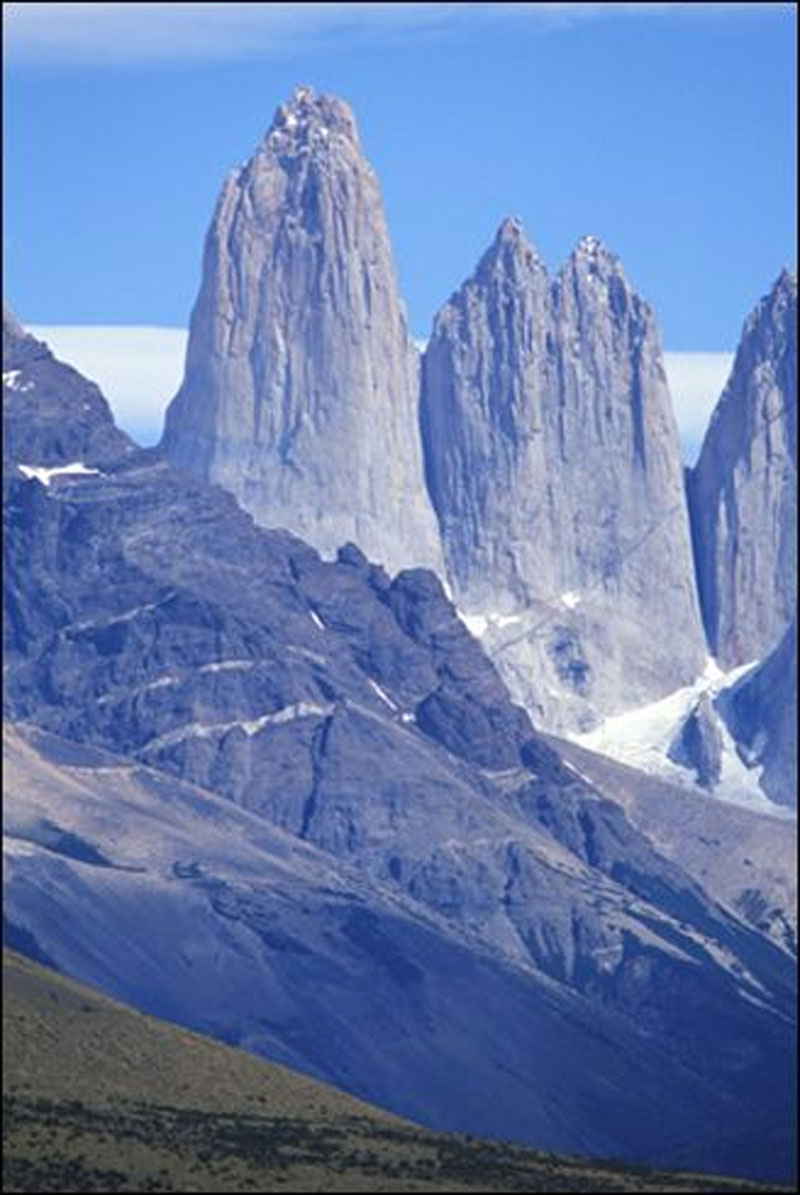
\includegraphics[width=\paperwidth,height=\paperheight]{watermark.jpg}%
	}
	\addtobeamertemplate{block begin}{\pgfsetfillopacity{0.8}}{\pgfsetfillopacity{1}}
\begin{document}
\begin{frame}{}
	\maketitle
\begin{columns}[T]
\begin{column}{.48\linewidth}
\begin{block}{Definition of the problem}
The general problem can be formalised this way.
Suppose we have some random variables $x\in\zR^p$ which correspond to
a mix of some primitive sources $s\in\zR^n$. The aim is to extract
from $x$ every source $s_i$. To do so, we suppose here that:\\
-- the sources are independents\\
-- the mix is linear and instantaneous\\
-- at most one source has a gaussian distribution.\\
We write:
\begin{equation}
 x = A s \ \ \mbox{and} \ \ y = W x,
\end{equation}

where $A$ is the mixing matrix, $W$ the separation matrix and $y$ the
estimation of the sources. The goal is then to find the matrix $W$ that
maximises the independence of $y$.
	 )
\end{block}
\begin{block}{Measure of independance}
As a measure of independence, we consider, for theoretical purpose,
the mutual information:\begin{equation}
\zZ IY = \int_{\zR^p} P(Y) \log\frac{P(Y)}{\prod_i P_i(Y_i)} \zdx Y.
\end{equation}
However, as it is too hard to compute, we consider other contrast functions, invariant by permutation, scaling on coordinates and maximal for independant ones.
For practical purpose, we consider other contrast function than the
mutual information (too hard to compute), which are invariant by permutation
and scaling on coordinates and ``minimal'' for independent coordinates.
\end{block}
\begin{block}{Results}
	\begin{figure}
	\hbox{\hspace{-.8cm}\begin{mygraph}{xmin=0, xmax=100, %
				                ymin=-1, ymax=1,%
								sizex=15, sizey=6}%
								{nomx=Sources, nomy=}%
	                	{0,50,100}{-1,-.5,...,1.05}%
	  \draw[zplot, red] plot file {data/init_sources_2.txt};
	  \draw[zplot, green!70!black] plot file {data/init_sources_3.txt};
	  \draw[zplot, blue] plot file {data/init_sources_1.txt};
	\end{mygraph}
	\hspace{-1cm}
	 \begin{mygraph}{xmin=0, xmax=100, %
	                 ymin=-1, ymax=1, %
	                sizex=15, sizey=6}%
	                {nomx=FastICA, nomy=}%
	                {0,50,100}{-1,-.5,...,1.05}
	  \draw[zplot, red] plot file {data/init_fast_1.txt};
	  \draw[zplot, green!70!black] plot file {data/init_fast_2.txt};
	  \draw[zplot, blue] plot file {data/init_fast_3.txt};
	\end{mygraph}\hss}
	\hbox{\hspace{-.8cm}\begin{mygraph}{xmin=0, xmax=100, %
	                 ymin=-1, ymax=1, %
	                sizex=15, sizey=6}%
	                {nomx=HJ, nomy=}%
	                {0,50,100}{-1,-.5,...,1.05}
	  \draw[zplot, red] plot file {data/init_hj_2.txt};
	  \draw[zplot, green!70!black] plot file {data/init_hj_1.txt};
	  \draw[zplot, blue] plot file {data/init_hj_3.txt};
	\end{mygraph}\hspace{-1cm}
	\begin{mygraph}{xmin=0, xmax=100, %
		                ymin=-1, ymax=1, %
		                sizex=15, sizey=6}%
		                {nomx=JADE, nomy=}%
		                {0,50,100}{-1,-.5,...,1.05}
		  \draw[zplot, red] plot file {data/init_jade_3.txt};
		  \draw[zplot, green!70!black] plot file {data/init_jade_1.txt};
		  \draw[zplot, blue] plot file {data/init_jade_2.txt};
		\end{mygraph}\hss}
		\vspace{-.2cm}
\caption{Results of the main ICA algorithms on simulated data. Each colour corresponds to a signal. The ``Sources'' graph shows the unmixed signal    s and the other ones the results of the algorithms. \label{fig:res}}
\end{figure}
\end{block}
\begin{block}{Kernel ICA}
	The idea here is to have a contrast function defined by the correlation of a range of functions over a function vector space $\mathcal{F}$. Thus defining the $\mathcal{F}$-correlation :
	\begin{equation*}
		\rho_{\mathcal{F}} (x_1,x_2) = \max\limits_{f_1,f_2 \in \mathcal{F}} \text{corr}(f_1(x_1),f_2(x_2))
	\end{equation*}
For $\mathcal{F}$ ``large enough'', we have the following equivalence : $\rho_{\mathcal{F}} (x_1,x_2) = 0 \Longleftrightarrow x_1 \ \& \ x_2$ are independant, hence the ``vector space contrast function'' idea.
	We then use the \textit{reproducing kernel Hilbert space} to obtain tractable computations over the vector space $\mathcal{F}$.
\end{block}

\begin{block}{Methods benchmark}
	We now wish to compare the different algorithms performing ICA we kept :\begin{itemize}
		\item HJ
		\item JADE
		\item FastICA
		\item KernelICA
\end{itemize}
One way to compare these algorithms is by their estimated mixing (ou unmixig) matrices : given numerous generated i.i.d. sources and a mixing matrix, all of these algorithms will return the best estimated mixing matrix according to their corresponding method.
Thus we could compare the estimations with our original mixing matrix with any norm whatsoever, but as we previously said, the algorithms are not able to find out the original order of the sources or their amplitude.
\end{block}
\end{column}

% Deuxième colonne
\begin{column}{.48\linewidth}
\begin{block}{Amari distance}
Fortunately, the ``Amari distance'' (which is unfortunately not a distance), gives a criterion of proximity between two matrices regardless to these two problems (amplitude and permutation).
If $U$ and $V$ are two $n$-by-$n$ matrices, the Amari distance is defined by:
\begin{equation*}
	d(U,V) = \frac{1}{2n}\sum\limits_{i=1}^n \left(\frac{\sum\limits_{j=1}^n|a_{ij}|}{\max_j |a_{ij}|}-1 \right)+\frac{1}{2n}\sum\limits_{j=1}^n \left(\frac{\sum\limits_{i=1}^n|a_{ij}|}{\max_i |a_{ij}|}-1 \right)
\end{equation*}
with $a_{ij} = (UV^{-1})_{ij}$. The closest it is to 0, the more $U$ and $V$ represents the same components.
\end{block}
\begin{block}{Modus operandi}
We will thereby analyze the results of the algorithms in terms of Amari distance over large number of i.i.d generated sources from several different distributions.
\end{block}
\begin{block}{Introduction}
\begin{itemize}
\item some items and $\alpha=\gamma, \sum_{i}$
\item some items
\item some items
\item some items
\end{itemize}
$\alpha=\gamma, \sum_{i}$
\end{block}
\begin{block}{Introduction}
\begin{itemize}
\item some items and $\alpha=\gamma, \sum_{i}$
\item some items
\item some items
\item some items
\end{itemize}
$\alpha=\gamma, \sum_{i}$
\end{block}
\begin{block}{Introduction}
\begin{itemize}
\item some items and $\alpha=\gamma, \sum_{i}$
\item some items
\item some items
\item some items
\end{itemize}
$\alpha=\gamma, \sum_{i}$
\end{block}
\begin{block}{Introduction}
\begin{itemize}
\item some items and $\alpha=\gamma, \sum_{i}$
\item some items
\item some items
\item some items
\end{itemize}
$\alpha=\gamma, \sum_{i}$
\end{block}

\begin{block}{Introduction}
\begin{itemize}
\item some items
\item some items
\item some items
\item some items
\end{itemize}
\end{block}
\begin{block}{Introduction}
\begin{itemize}
\item some items and $\alpha=\gamma, \sum_{i}$
\item some items
\item some items
\item some items
\end{itemize}
$\alpha=\gamma, \sum_{i}$
\end{block}
\begin{block}{Introduction}
\begin{itemize}
\item some items and $\alpha=\gamma, \sum_{i}$
\item some items
\item some items
\item some items
\end{itemize}
$\alpha=\gamma, \sum_{i}$
\end{block}

\end{column}
\end{columns}

\end{frame}
\end{document}
